\documentclass[11pt]{article}
\usepackage[margin=20mm,headheight=16pt]{geometry}
\usepackage[table]{xcolor}
\usepackage{graphicx,amsmath,amssymb,booktabs,longtable,array,tabularx,multirow,siunitx}
\usepackage{fancyhdr,titlesec,enumitem,caption,float,lastpage}
\usepackage{tikz,pgfplots}
\usetikzlibrary{arrows.meta,positioning,calc,fit,backgrounds,shapes.geometric,matrix,trees,patterns,decorations.pathreplacing}
\usepgfplotslibrary{fillbetween,statistics,groupplots}
\pgfplotsset{compat=1.18}
\usepackage{hyperref}
\pagestyle{fancy}\fancyhf{}\fancyhead[L]{Synthetic diagrams}\fancyfoot[R]{\thepage\ / \pageref{LastPage}}
\titleformat{\section}{\large\sffamily\bfseries\color{blue}}{\thesection}{1em}{}
\setlist{itemsep=2pt}
\begin{document}
{\sffamily\tiny S\scriptsize S\footnotesize S\small S\normalsize S\large S\Large S\LARGE S\huge S\Huge S}\par
{\sffamily\bfseries\tiny B\scriptsize B\footnotesize B\small B\normalsize B\large B\Large B\LARGE B\huge B\Huge B}\par
{\sffamily\itshape I\bfseries B}\par
\section{Synthetic diagrams, styled tables and numeric formatting}
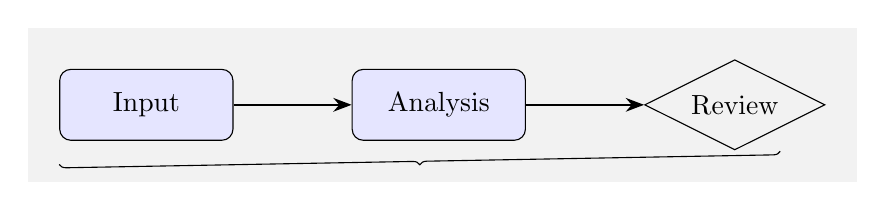
\begin{tikzpicture}[node distance=15mm,box/.style={draw,rounded corners,fill=blue!10,minimum width=22mm,minimum height=9mm},>=Stealth]
\node[box] (input) {Input};
\node[box,right=of input] (analysis) {Analysis};
\node[diamond,aspect=2,draw,right=of analysis] (decision) {Review};
\draw[->,thick] (input)--(analysis);
\draw[->,thick] (analysis)--(decision);
\draw[decorate,decoration={brace,mirror}] ($(input.south west)+(0,-.3)$)--($(decision.south east)+(0,-.3)$);
\begin{scope}[on background layer]\node[fill=gray!10,fit=(input)(analysis)(decision),inner sep=4mm] {};\end{scope}
\end{tikzpicture}
\begin{table}[H]\centering\caption{Synthetic comparison}
\rowcolors{2}{gray!10}{white}
\begin{tabularx}{\linewidth}{lXS}\toprule Category & Evidence & {Value}\\\midrule
\multirow{2}{*}{Example} & Synthetic data only & 1234.56\\ & Measured observation & 42.50\\\bottomrule
\end{tabularx}\end{table}
Units: \num{12345.67}\,\si{\kilo\metre}. $\mathbb{R}\quad\sum_{i=1}^3 i=6$.
\begin{itemize}[label=\textbullet]\item Synthetic list\end{itemize}
\begin{longtable}{lr}\toprule Item & Count\\\midrule A & 1\\ B & 2\\\bottomrule\end{longtable}
\section{Synthetic graphs}
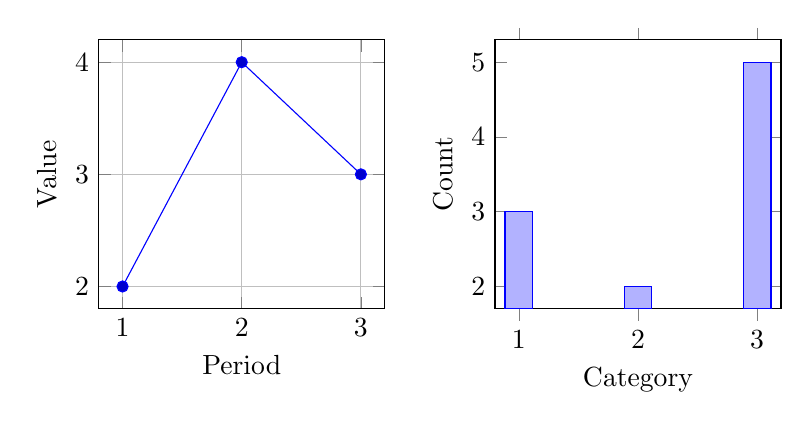
\begin{tikzpicture}
\begin{groupplot}[group style={group size=2 by 1,horizontal sep=14mm},width=.43\linewidth,height=50mm]
\nextgroupplot[xlabel=Period,ylabel=Value,grid=major]
\addplot+[mark=*] coordinates {(1,2)(2,4)(3,3)};
\nextgroupplot[ybar,xlabel=Category,ylabel=Count,xtick={1,2,3}]
\addplot+[fill=blue!30] coordinates {(1,3)(2,2)(3,5)};
\end{groupplot}
\end{tikzpicture}
\newpage
\section{Synthetic scatter, area and statistical plots}
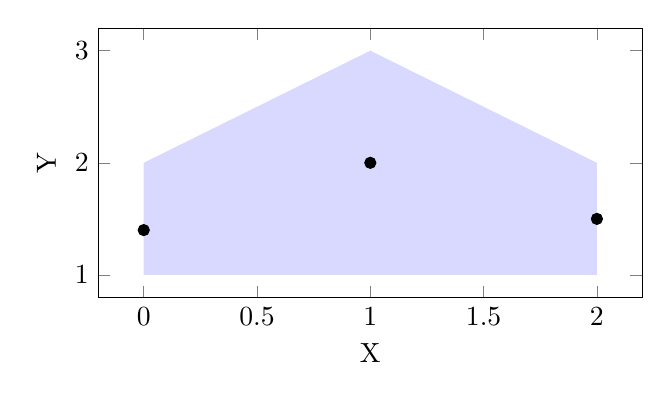
\begin{tikzpicture}\begin{axis}[width=.7\linewidth,height=50mm,xlabel=X,ylabel=Y]
\addplot[name path=upper,draw=none] coordinates {(0,2)(1,3)(2,2)};
\addplot[name path=lower,draw=none] coordinates {(0,1)(1,1)(2,1)};
\addplot[fill=blue!15] fill between[of=upper and lower];
\addplot[only marks,mark=*] coordinates {(0,1.4)(1,2)(2,1.5)};
\end{axis}\end{tikzpicture}\par
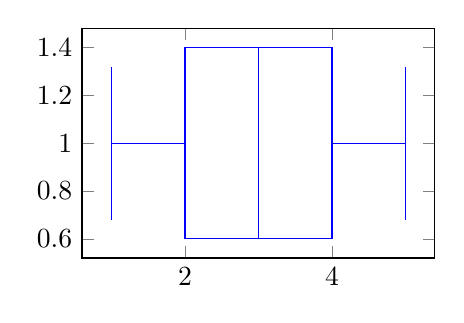
\begin{tikzpicture}\begin{axis}[width=.5\linewidth,height=45mm]
\addplot+[boxplot prepared={lower whisker=1,lower quartile=2,median=3,upper quartile=4,upper whisker=5}] coordinates {};
\end{axis}\end{tikzpicture}
\href{https://example.com}{Synthetic reference}
\end{document}
